\documentclass[11pt]{article}

\usepackage{graphicx}

% graphicx points to my assets folder with all the images.
\graphicspath{ {assets/} }

% Use wide margins, but not quite so wide as fullpage.sty
\marginparwidth 0.5in 
\oddsidemargin 0.25in 
\evensidemargin 0.25in 
\marginparsep 0.25in
\topmargin 0.25in 
\textwidth 6in \textheight 8 in
% That's about enough definitions


\begin{document}
\hfill\vbox{\hbox{Jude Shin}
		\hbox{Cpe 453, Section 01}	
		\hbox{Lab 5}	
		\hbox{\today}}\par

\bigskip
\centerline{\Large\bf Lab 5: Problem Set}\par
\bigskip

\section*{Solutions}
\begin{enumerate} 
	\item Each program has a 50/50 chance of either waiting on I/O, or doing work (using the CPU or not using the CPU). When the CPU is idle, that means all 4 of the programs will be waiting on I/O at the same time (they are all not using the CPU at the same time). If there was one program, then the probability of the CPU being idle would be the same as the chances of the program waiting on I/O (which is 50\%). If there were two processes, the chances would multiply ($0.50 * 0.50 = 0.25$). If we extrapolate this pattern to 4 processes, then the odds of each program waiting for I/O at the same time would be 6.25\% ($0.5 * 0.5 * 0.5 * 0.5 = 0.0625$). If all I/O operations are distributed randomly with even probability, this would mean that out of the whole time that the CPU is trying to run these 4 programs, the CPU would be idle 6.25\% of that time. 
	\item
		\begin{enumerate}
			\item The virtual address of 20 is 20 bytes away from the start of the virtual page in the range 0K-4K. This means that it will be 20 bytes away from the associated page in the physical memory. The virtual page 0K-4K maps to the physical page 8K-12K. The virtual address 20 will be mapped to the physical address 8020.
			\item The virtual address of 4100 is 100 bytes away from the start of the virtual page in the range 4K-8K. This means that it will be 100 bytes away from the associated page in the physical memory. The virtual page 4K-8K maps to the physical page 4K-8K. The virtual address 4100 will be mapped to the physical address 4100.
			\item The virtual address of 8300  is 300 bytes away from the start of the virtual page in the range 8K-12K. This means that it will be 300 bytes away from the associated page in the physical memory. The virtual page 8K-12K maps to the physical page 24K-28K. The virtual address 8300 will be mapped to the physical address 24300.
		\end{enumerate}
	\item There are 32 bits in an address total. If 9 are used to locate the top level page table field, and 11 bits are used to reference the second level page table field, then there are only 12 remaining bits left to search within that page. ($32 - 9 - 11 = 12$). If we only have 12 bits to search through the page, there can only be $2^{12}$ bits total. This allows us to locate the particular page, as well as look at a particular bit of the page. Therefore, there are only 4096 bits in one page. ($2^{12} = 4096 = 4KB$). 

		To calculate the number of pages in the address space, we can only have 9+11 bits to identify a page. This leaves us with 2\^20 unique page tables that we can use. ($2^{9+11} = 2^{20} = 1048576$).
	\item
		\begin{enumerate}
			\item NRU stands for ``Not Recently Used", which means that it will replace the lowest-numbered non-empty class (if there are multiple in the same class, it chooses at random). The classes are defined as follows: 

				{\tt Class 0: not referenced, not modified.

				Class 1: not referenced, modified.

				Class 2: referenced, not modified.

				Class 3: referenced, modified.}


				This means that Page 0 (the one that has not been referenced, nor modified at the time of loading) will be chosen to be replaced.
			\item FIFO stands for ``First In First Out", which means it will replace the oldest page in terms of when it was loaded. Page 2 was loaded 120 clock ticks from the beginning (of time I suppose). This means that it was loaded the earliest, and will be replaced.
			\item LRU stands for ``Last Recently Used", which means that it will replace the page that was accessed the longest time ago (aka, the Last Ref. value will be lower). Page 1 has the lowest Last Ref. time, therefore this page will be picked to be replaced. 
			\item ``Second Chance" is a page replacement algorithm that is a slight modification to the FIFO algorithm. It replaces the oldest page (just like FIFO), however, when the oldest page is chosen, it takes a look at the R bit. If the R bit is set to 1, that means that it was referenced recently, so set the R bit to 0 and put it in the back of the queue of pages to search. Continue the search through the pages from oldest to newest. If we find an old page where the R bit is set to 0, then feel free to replace the page. 

				In our case, page 2 was the oldest page, but it had an R bit set. Put it to the back of the line an look at the next oldest page, which is page 0. page 0's R bit is not set, therefore it is chosen to be replaced.
		\end{enumerate}
	\item The string reference string ``0713272013" represents the pages that is requested. (First request page 0, then request page 7, then request...). Remember that a ``page" represents the block of virtual memory, and a ``frame" represents a block in the physical memory. If we have 8 pages, and 4 frames, we really only physically have 4 frames, and there will have to be some pages that are replaced. The 4 values inside of the brackets $[]$ will represent the physical frames that we have on RAM. 

		\begin{enumerate}
			\item $[-, -, -, -]$ \textrightarrow $[0, -, -, -]$: Page 0 is requested. Since all 4 of the frames are empty, there is no page loaded in a frame. A page fault occurs and loads page 0 in a frame. The number of page faults that have occurred at this point is 1.
			\item $[0, -, -, -]$ \textrightarrow $[0, 7, -, -]$: Page 7 is requested. Page 7 is not in a frame (just like above), so a page fault occurs. The number of page faults that have occurred at this point is 2.
			\item $[0, 7, -, -]$ \textrightarrow $[0, 7, 1, -]$: Page 1 is requested, and a page fault occurs. The number of page faults that have occurred at this point is 3.
			\item $[0, 7, 1, -]$ \textrightarrow $[0, 7, 1, 3]$: Page 3 is requested, and a page fault occur. The number of page faults that have occurred at this point is 4.
		\item $[0, 7, 1, 3]$ \textrightarrow $[2, 7, 1, 3]$: Page 2 is requested, but there are no empty frames, nor are there any frames that currently hold page 2. A page fault occurs. Using FIFO, the oldest page will be replaced. In this case, page 0. The number of page faults that have occurred at this point is 5.
			\item $[2, 7, 1, 3]$ \textrightarrow $[2, 7, 1, 3]$: Page 7 is requested, but it is already loaded in a frame! Do nothing and be happy.
			\item $[2, 7, 1, 3]$ \textrightarrow $[2, 7, 1, 3]$: Page 2 is requested, but it is already loaded in a frame! Do nothing and be happy.
			\item $[2, 7, 1, 3]$ \textrightarrow $[2, 0, 1, 3]$: Page 0 is requested, but there are no empty frames, nor are there any frames that currently hold page 0. A page fault occurs. Using FIFO, the oldest page will be replaced. Page 2 was just requested, and page 7 was loaded at the very beginning. In this case, the oldest page is 7. The number of page faults that have occurred at this point is 6.
			\item $[2, 0, 1, 3]$ \textrightarrow $[2, 0, 1, 3]$: Page 1 is requested, but it is already loaded in a frame! Do nothing and be happy.
			\item $[2, 0, 1, 3]$ \textrightarrow $[2, 0, 1, 3]$: Page 3 is requested, but it is already loaded in a frame! Do nothing and be happy.
		\end{enumerate}

		After everything is said and done, there were 4 page faults in the beginning, and 2 extra page faults (one at step 5, and one at step 8). In total there were 6 page faults using FIFO.

	\item Using the same reference string in problem 5, ``0713272013", But this time with LRU, the page faults might be different. 

		\begin{enumerate}
			\item $[-, -, -, -]$ \textrightarrow $[0, -, -, -]$: Page 0 is requested. Since all 4 of the frames are empty, there is no page loaded in a frame. A page fault occurs and loads page 0 in a frame. The number of page faults that have occurred at this point is 1.
			\item $[0, -, -, -]$ \textrightarrow $[0, 7, -, -]$: Page 7 is requested. Page 7 is not in a frame (just like above), so a page fault occurs. The number of page faults that have occurred at this point is 2.
			\item $[0, 7, -, -]$ \textrightarrow $[0, 7, 1, -]$: Page 1 is requested, and a page fault occurs. The number of page faults that have occurred at this point is 3.
			\item $[0, 7, 1, -]$ \textrightarrow $[0, 7, 1, 3]$: Page 3 is requested, and a page fault occur. The number of page faults that have occurred at this point is 4.
			\item $[0, 7, 1, 3]$ \textrightarrow $[2, 7, 1, 3]$: Page 2 is requested, but there are no empty frames, nor are there any frames that currently hold page 2. A page fault occurs. Using LRU, the least recently used page will be replaced. In this case, the time that they were last used was the time that they were also loaded. Page 0 is replaced as it was the oldest to be referenced. The number of page faults that have occurred at this point is 4.
			\item $[2, 7, 1, 3]$ \textrightarrow $[2, 7, 1, 3]$: Page 7 is requested, but it is already loaded in a frame! Do nothing and be happy.
			\item $[2, 7, 1, 3]$ \textrightarrow $[2, 7, 1, 3]$: Page 2 is requested, but it is already loaded in a frame! Do nothing and be happy.
			\item $[2, 7, 1, 3]$ \textrightarrow $[2, 7, 0, 3]$: Page 0 is requested, but there are no empty frames, nor are there any frames that currently hold page 0. A page fault occurs. Using LUR, the least recently used page will be replaced. Page 2 was just requested, and page 7 was also requested just before that! Pages 1 and 3 are the least recently used ones, but since page 1 was added first, it is technically older than page 3, so it is chosen. The number of page faults that have occurred at this point is 6.
			\item $[2, 7, 0, 3]$ \textrightarrow $[2, 7, 0, 1]$: Page 1 is requested, but there are no empty frames, nor are there any frames that currently hold page 1. A page fault occurs. Using LUR, the least recently used page will be replaced. Page 0 was just updated, before that was page 2, and before that was page 7. This leaves us with page 3 as being the oldest one requested, therefore, it is chosen to be replaced. The number of page faults that have occurred at this point is 7.
			\item $[2, 7, 0, 1]$ \textrightarrow $[2, 3, 0, 1]$: Page 3 is requested, and a page fault occurs. I can't help you if you don't know what goes on here, and I am not going to spell it out again. The oldest page here is 7. It is chosen for a page fault. The number of page faults that have occurred at this point is 8.
		\end{enumerate}

		After everything happens, there are 4 page faults for the beginning, and then 4 more page faults in later steps. In total there were 8 page faults using LRU.

	\item 
		If in the 60 seconds there were 15,000 page faults, then out of those 60 seconds, $(2,000 microseconds * 15,000 = 30,000,000 microseconds = 30.000s)$ would be spent handling the page faults. The remaining 30 seconds would be the time the program actually takes. If the memory was doubled, then there would be half as many page faults that will occur, so the original 15,000 page faults would get cut in half to 7,500 page faults.
		If it takes 2,000  microseconds to handle a page fault, and there now only being 7,500 page faults because of the doubled memory, the total time spent handling the page faults would be $2,000 microseconds * 7,500 = 15,000,000 microseconds$. Adding that to the raw time the program takes to execute (which was 30,000,000 microseconds) would leave us with 45,000,000 microseconds, or 45 seconds in total.

	\item A directory entry is a struct that holds an inode number, and then a name that is associated with it. This means that the actual data is not stored within the directory inode, rather pointers to inodes that do have the data. Reading a directory would mean going through the zones and reading those directory entry structs. In comparison, reading a regular file would be reading the data in the zones with no structs. ``Read the raw directories"is an ambiguous term. 

	\item The hit rate $h$ is the number of blocks found in the cache. If there is 1 block in the cache and 4 total blocks on the disk, then the hit rate is 0.25. That means that the ``not hit rate" is $1-h$; in our example, the ``not hit rate" would be 0.75. 

		If {\tt h} is 0, then there is no chance that there is a block in the cache. The block will always be read from the disk. This end of the plot should show a mean time of 40ms. On the other hand, if {\tt h} is 1, then there will always be a hit, so the plot should show a mean time of 10ms. Let's say that {\tt h} is 0.5. That means that 1/2 of the requests are handled with the cache, and 1/2 of them are handled with the disk. Just multiply the hit rate with the hit time to get the mean time. 

		If you multiply the time per request with the rate, you can get the mean time. The following formula can be used to represent the overall mean time. This formula can be seen in Figure \ref{fig:graph}.

		$T(h) = (40ms)*(1-h) + (1ms)*(h)$ \textrightarrow 

		$T(h) = (40)*(1-h) + h$ \textrightarrow 

		$T(h) = (40-40h) + h$ \textrightarrow 

		$T(h) = 40 - 39h$ 

    \begin{figure}[htbp]
        \centering
        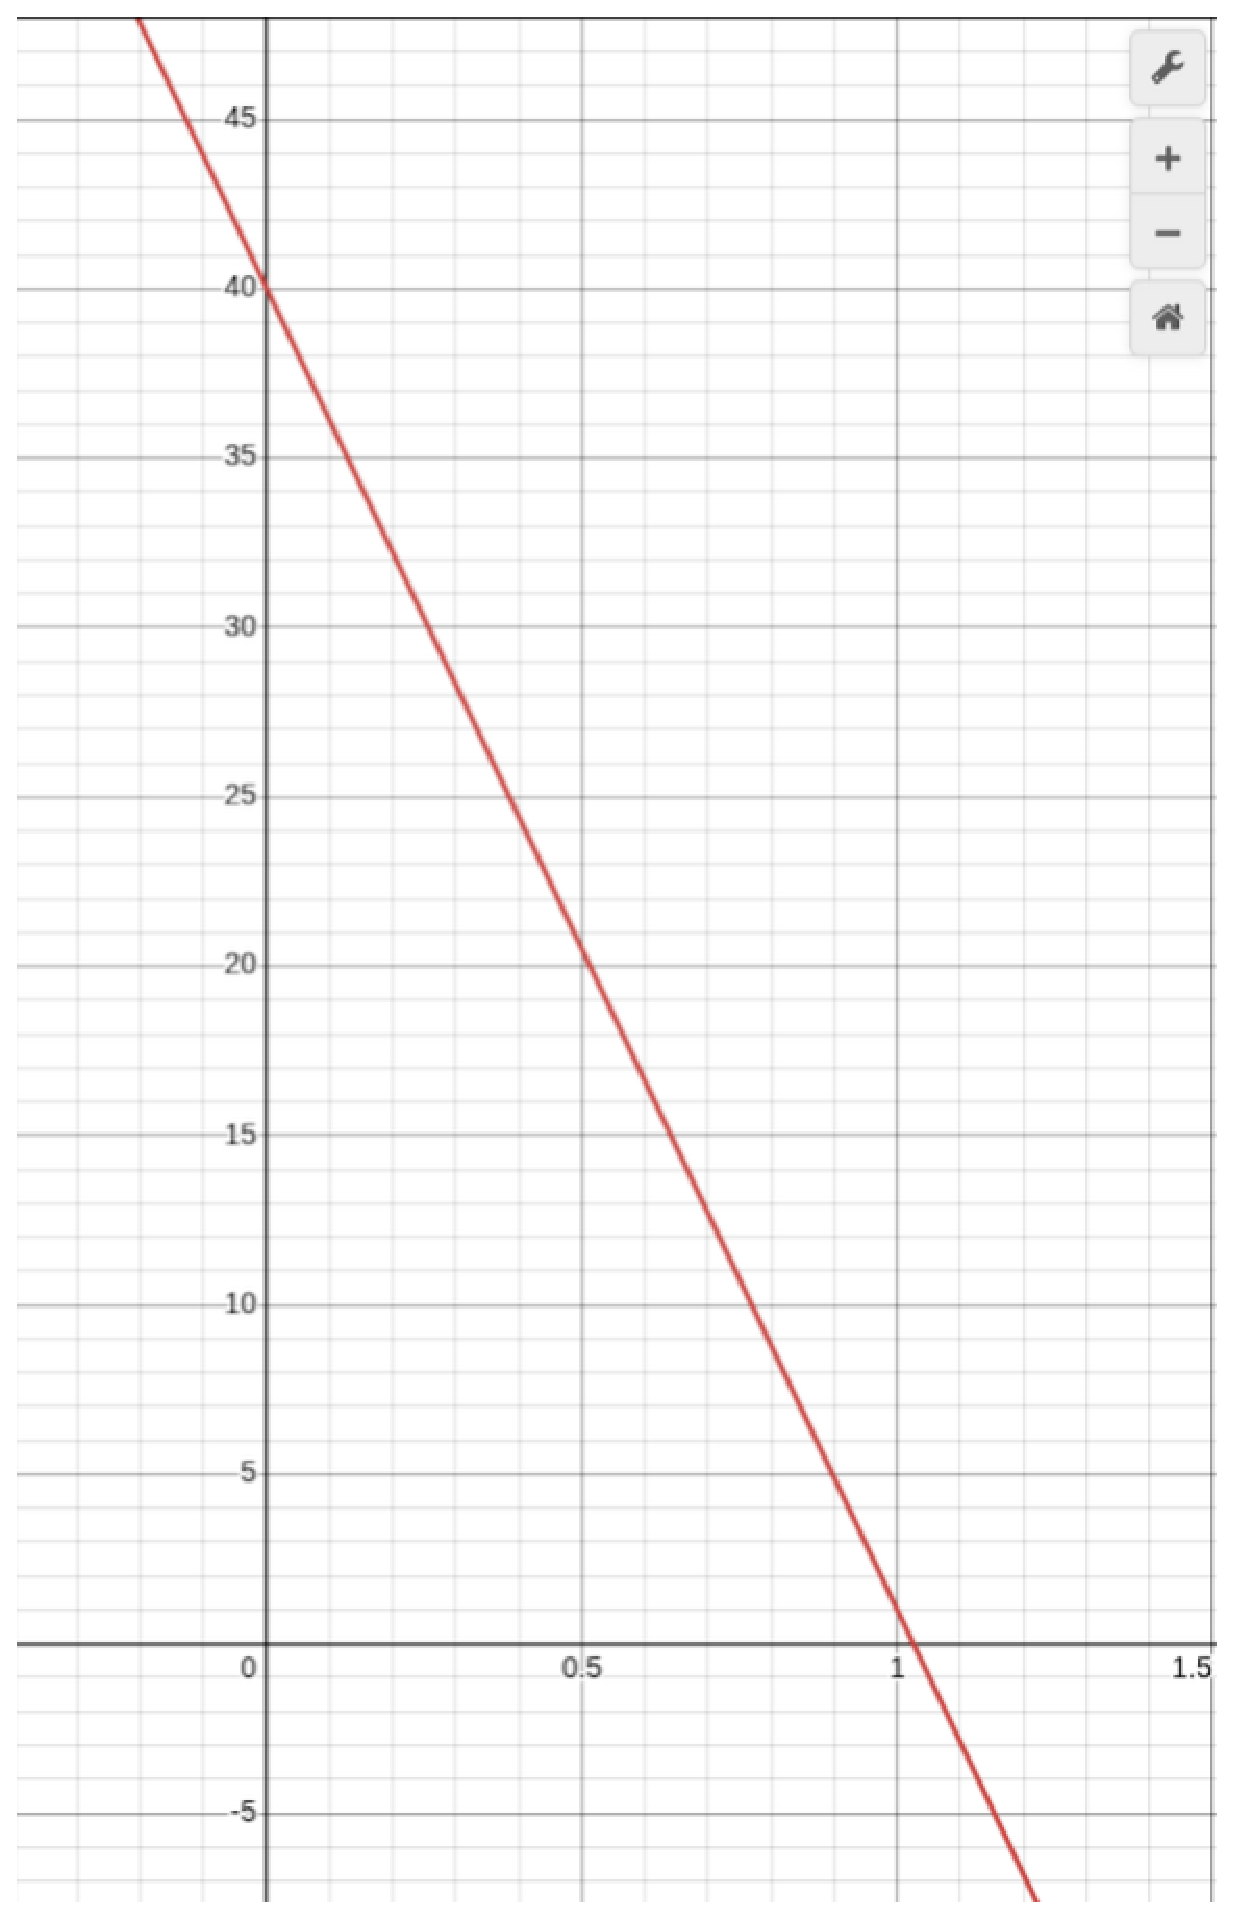
\includegraphics[width=0.8\linewidth]{hitrate}
        \caption{x-axis representing h in the domain of $[0, 1]$, and the y axis representing the mean time in milliseconds}
        \label{fig:graph}
    \end{figure}

	\item
	\item
	\item
\end{enumerate} 
\end{document}
